\documentclass{article}

\usepackage{amsmath}
\usepackage{url}
\usepackage{graphicx}

\newcommand{\newword}[1]{{\bf #1}}
\newtheorem{problem}{Problem}
\newcommand{\NP}{\ensuremath{\mathcal{NP}}}

\title{Using Cell Phone Keyboards is (\NP) Hard}
\author{P. Boothe}

\begin{document}
\maketitle

\begin{abstract}
Sending text messages on cell phones which only contain the keys 0-9 and \# and
* can be a painful experience.  We consider the problem of designing an optimal
mapping of numbers to sets of letters to act as an alternative to the standard
$\{2\to\{abc\}, 3\to\{def\}\ldots\}$.  Our overall goal is to minimize the
number of buttons that must be pressed to enter an aferage message in English.
We prove that the problem in almost all of its variations is \NP hard, but
describe several mappings which improve the standard one.  With luck, one of
these new mappings will achieve success similar to that of the Dvorak layout
for computer keyboards.
\end{abstract}

Typing on a keyboard which has fewer keys than there are letters in the
alphabet can be a painful task.  There are a plethora of input schemes which
attempt to make this task easier, but the one thing they all have in common is
that all of these input methods use the standard mapping of numeric keys to
alphabetic numbers of 
$\{2\to\{abc\},
         3\to\{def\}, 4\to\{ghi\}, 5\to\{jkl\}, 6\to\{mno\}, 7\to\{pqrs\},
         8\to\{tuv\}, 9\to\{wxyz\}\}$.
However, if we don't mind breaking some ``legacy'' applications of the phone
system such as ``1-800-FLOWERS'', then we might try rearranging the numbers on
the keys to make messages easier to type.  Most variants of this problem turn
out to be NP-hard, unfortunately.

Before we get any farther, let us sketch the basic problem that we will keep
revising and revisiting throughout this paper.
\begin{problem}[{\sc MinimumKeystrokes}]~\\
{\sc Instance}: A set of letters corresponding to an alphabet $A$ $(|A| =
n)$, a number of keys $k$, an input method $IN$, and a set of
tuples of words and frequencies $W$.  The frequencies in $W$ are integers,
and the words are made up of solely of elements of $A$.  We will
treat $IN$ as a function which, given a partition of $A$ and a word
$w$, returns how many keystrokes are required to type $w$.~\\
        ~\\
{\sc Question}: What is the best partition of $A$ into $k$ sets, such that the
total number of keystrokes to type every word in $W$ its associated frequency
times is minimized?  Equivalently, what is the partition of $P$ of $A$ ($|P| = k$) that
will minimize
$$\sum_{(w,f)\in W} f*IN(w,P)$$
\label{probtemplate}
\end{problem}

Over the course of this paper we consider three different real-world
schemes for $IN$ (basic typing, T9, and predictive T9), and for each
variant that is proven \NP-hard, we consider the restriction on $P$ that
requires that we keep the alphabet in alphabetical order.  In all cases
where it is computationally feasible we provide results for the case of
the English language, on 8-key keyboards, using the British National
Corpus\cite{bnc}.  

\section{Setting a Baseline and Solving the Easiest Problem}

The baseline we compare against is the most painful method of text entry.  I
imagine that no ``digital native'' actually uses this input method, and that it
is available on all phones solely that their parents might use it.  In this
method, to type an `a', the user of the cellphone types the `2' key; to type a
`b' they type `22', to type `c' they type `222', to type a `d' they type `3',
to type an `e' they type `33', and so on.  To type a word with multiple
letters that use the same key, such as `accept', the user must pause
between keystrokes.  Thus, the full key entry sequence for `accept', using
`.' to indicate a pause, is `2.22.223378'.

\begin{figure}
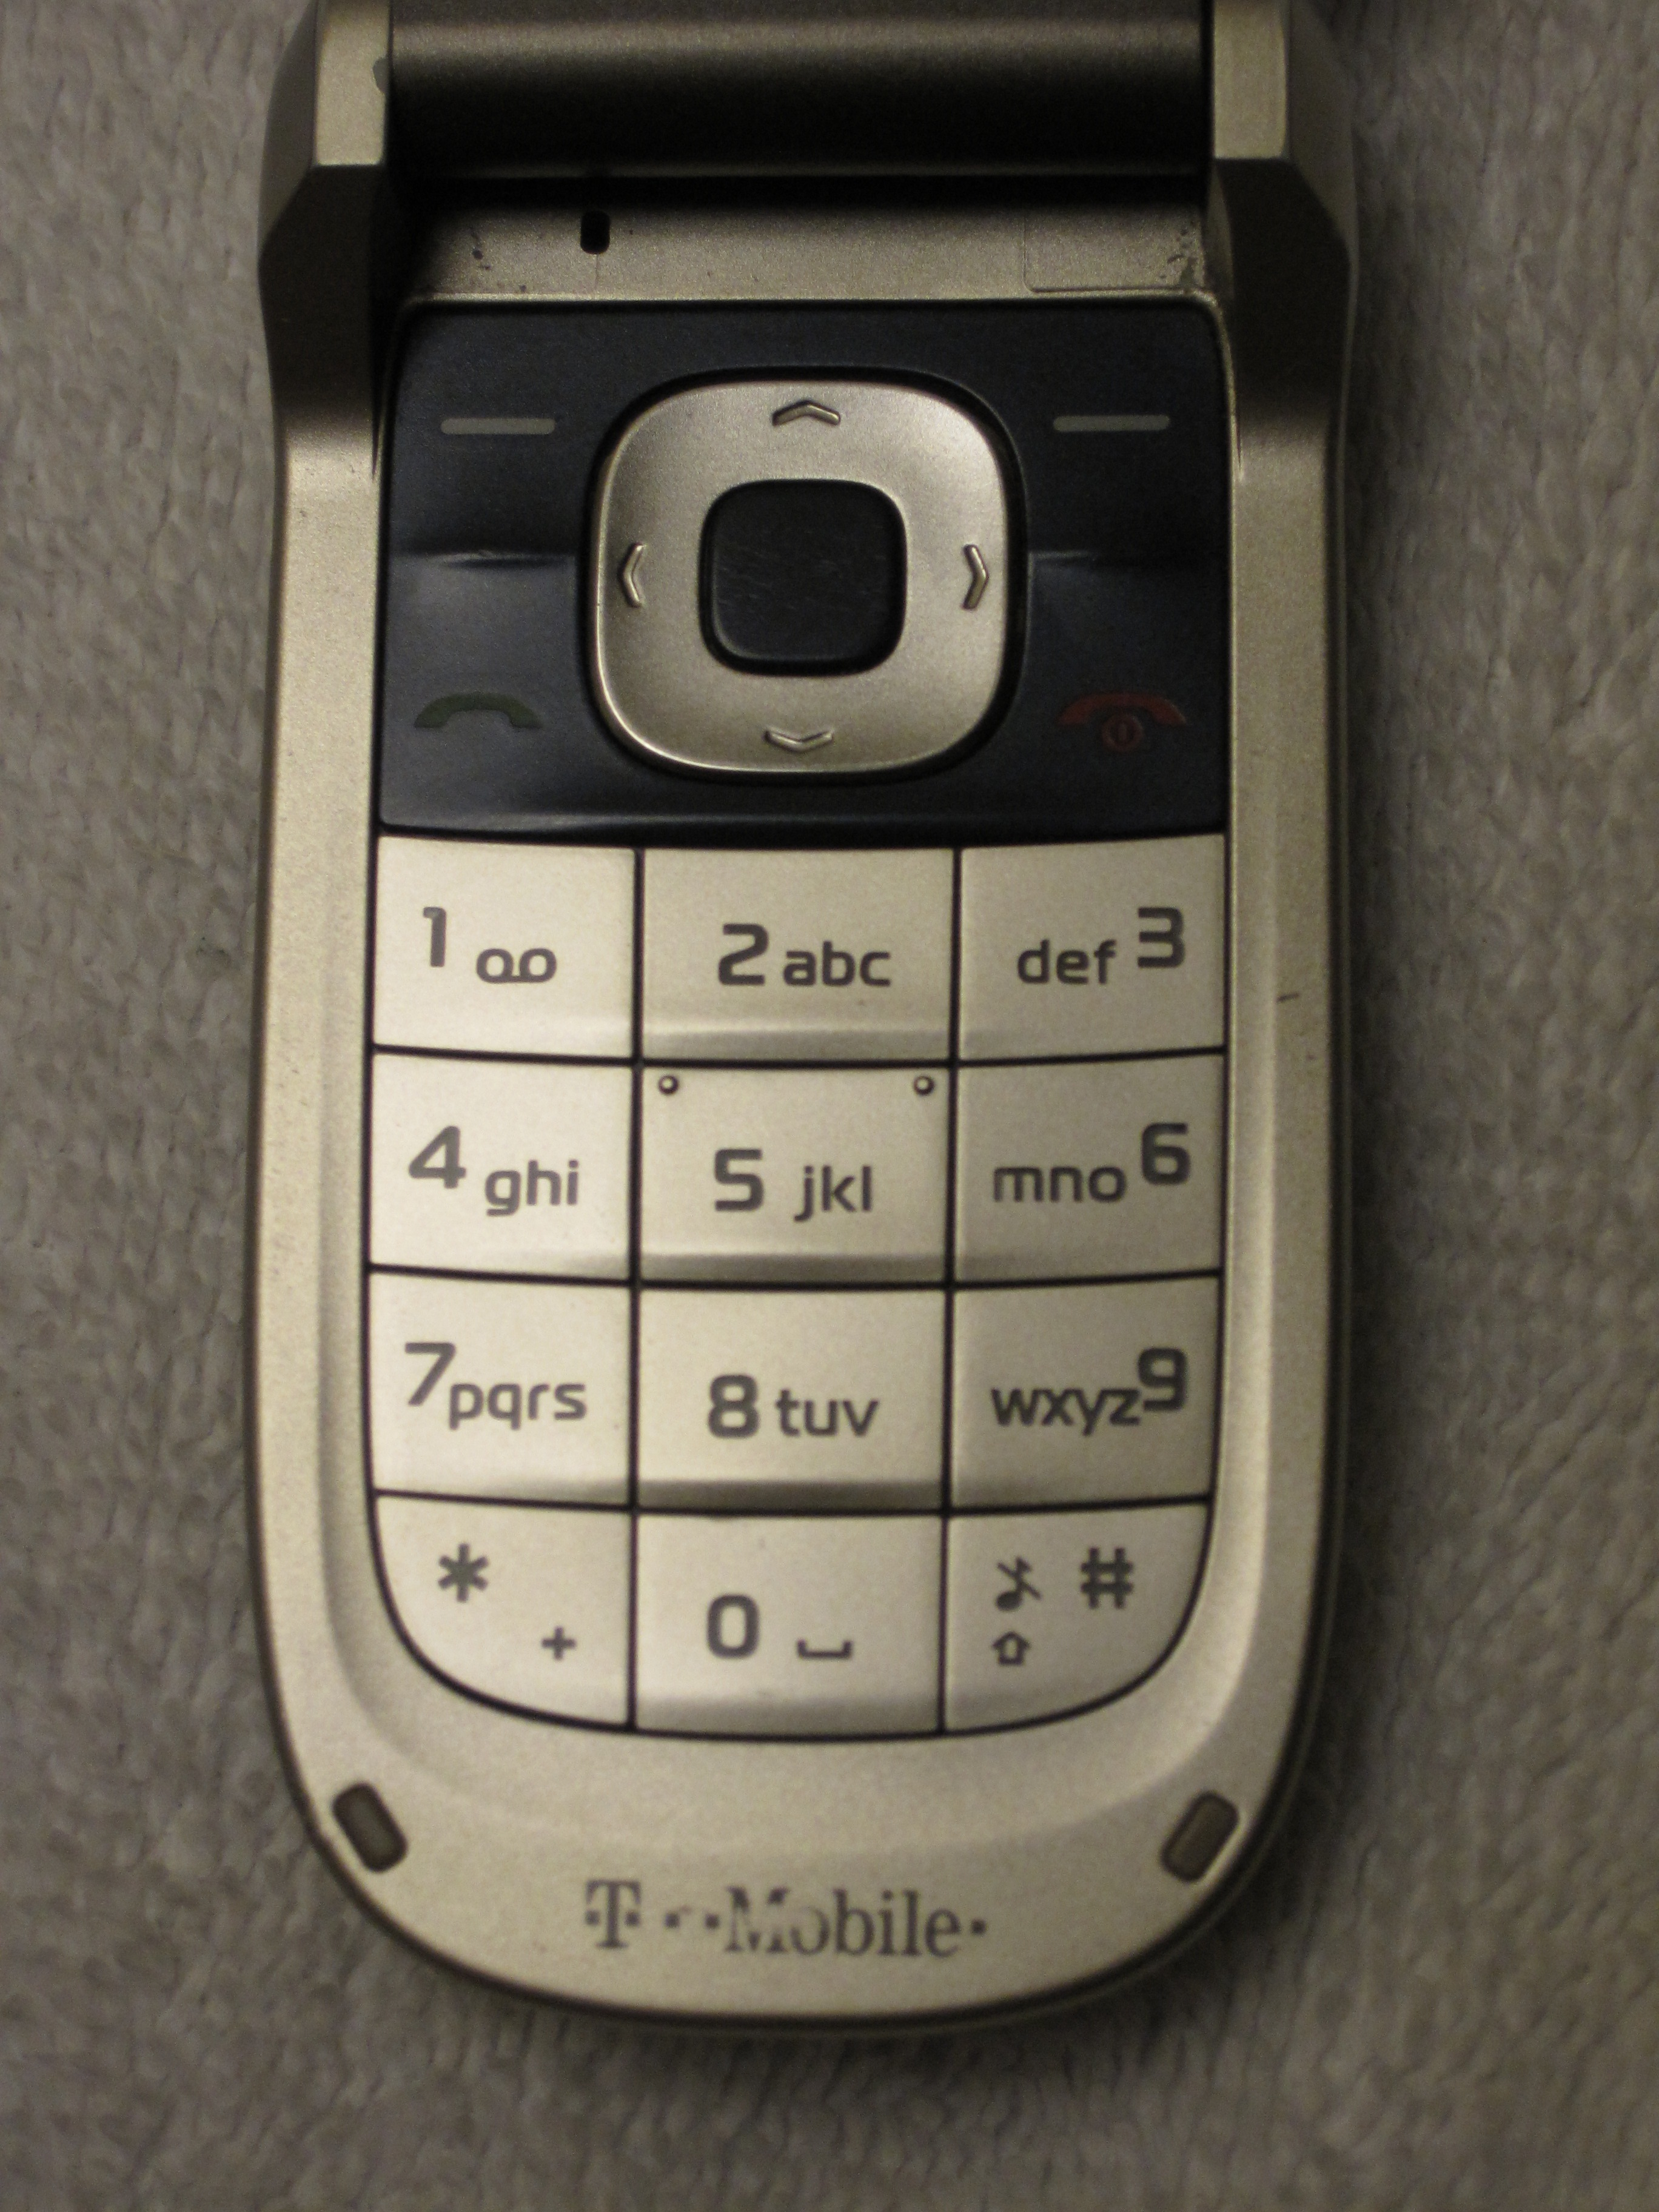
\includegraphics[width=2in]{phonekeys.jpg}
\caption{A cell phone keyboard}
\label{keypic}
\end{figure}

Initially, we will completely neglect the pauses and concern ourselves solely
with the number of keystrokes required.  This implies that `a' will always
require one button press, `b' will always require two, and so on.  Thus, to get
a baseline of how many keystrokes are required to enter the entirety of our
corpus of words $W$, we count the total number of occurences of each letter,
and multiply that number of occurrences by the number of button pushes
required by that letter.  Running this on the British National Corpus
using the standard cell phone keyboard layout, we find that entering the
entirety of the 100,106,029 word occurrences in the corpus would require
948,049,046 button presses.  

If we examine a cell phone keyboard (Figure~\ref{keypic}) then we can see that
there are some terrible choices being made.  The frequently-occurring letters
'r' and 's' require more keystrokes than 'q'!  Surely, a better designed
keyboard can do better than this.  If we just reversed the order of the letters
on the 7 key, from `pqrs' to `srqp', the number of button presses required
would drop to 865,118,331 --- a savings of more than $8.7\%$!  If we assume
that every button press takes an equal amount of time, then this corresponds
the users spending $8.7\%$ less time entering their text messages.  In an
effort to find out how low this can go, we define the problem {\sc
BasicCellPhoneTyping} based on the template problem on
page~\pageref{probtemplate}.

\bibliographystyle{abbrv}
\bibliography{bibliography}
\end{document}
